\documentclass[a4paper]{article}
\usepackage{amsmath}
% \usepackage{stmaryrd}
\usepackage[margin=1.5cm]{geometry}
\usepackage{amsthm}
\usepackage{amssymb}
\usepackage{graphicx}
\usepackage{hyperref}
\usepackage{xfrac}
\usepackage{listings}
\usepackage{enumitem}
\usepackage{array}
\usepackage{changepage}
\usepackage{pgfplots}
\lstset{language=C}
\usepackage[latin1]{inputenc}

\newcommand{\miniitem}[1]{\begin{itemize}\item #1\end{itemize}}

\newenvironment{redmatrix}
  {\left(\array{@{}rrr|c@{}}}
  {\endarray\right)}
\newenvironment{ropmatrix}
  {\array{@{}c@{}}}
  {\endarray}
\newcommand\opone[2]{\xrightarrow{(#1)\times r_#2}}
\newcommand\optwo[3]{\xrightarrow{r_#1{}-{} #2r_#3}}

\newcommand{\ansline}{\begin{center}\rule{8cm}{0.4pt}\end{center}}

\pgfplotsset{compat=1.16}

\setlength\parindent{0pt}

\setlist[description]{leftmargin=1cm,labelindent=1cm}

\title{COMP4121 Notes}
\author{Charlie Bradford}
\date{\today}

\begin{document}
\maketitle

%\section{PageRank}


\section{Iterative Filtering}


\subsection{Reciprocal}
Define the \textit{dist} at iteration $p$ of a sensor $j$ as the square euclidean sum of all its measurements and the \textit{est} at iteration $p-1$ of the true value.
\begin{align*}
	\textit{dist}^{(p)}(j)\ &=\ \sum\limits_{k=1}^{i}(m(j,k)-\textit{est}^{(p-1)})^2 \\
	\textit{weight}^{(p)}(j)\ &= \frac{\frac{1}{\textit{dist}^{(p)}}}{\sum\limits_{k=1}^{i}\frac{1}{\textit{dist}^{(p)}(k)}} \\
	\textit{est}^{(p+1)}\ &= \sum\limits_{k=1}^{i}\textit{weight}^{(p)}(j)*m(j)
\end{align*}


\subsection{Affine}

\textit{est} and \textit{dist} are as above, however \textit{weight} is defined as:
\begin{align*}
	w^{(p)}(j)\ &=\ \textit{max}\ \textit{dist}^{(p)}(k) - \textit{dist}(j) \\
	\textit{weight}^{(p)}(j)\ &=\ \frac{w^{(p)}(j)}{\sum\limits_k w^{(p)}(k)}
\end{align*}


\subsection{UNSW}
Defining $L(i,k,j)$ as the likelihood of measurements of sensor $j$ to be correct from the point of view of sensor $k$ at instant $i$ (assuming Gaussian distribution).
$$L(k,j,i)\ =\ \frac{1}{\sqrt{2\pi*V_k}}e^{-\frac{(m(j,i)-m(k,i))^2}{2V_k}}$$
Now derive $\hat{L}(k,j)$ as the trustworthiness of sensor $j$ from the point of view of sensor $k$ across all instants.
$$\hat{L}(k,j)\ =\ \Pi\frac{1}{\sqrt{2\pi*V_k}}e^{-\frac{(m(j,i)-m(k,i))^2}{2V_k}}\ =\ (2\pi*V_k)^{\frac{T}{2}}e^{-\sum\frac{(m(j,i)-m(k,i))^2}{2V_k}}$$
This leaves $\tilde{L}(j)$ as the trustworthiness of $j$ in general.
$$\tilde{L}(j)\ =\ \Pi L(k,j)$$


\section{Recommender Systems}


\subsection{Neighbourhood Method}
Figure out the taste of each user that is independent of:
\begin{itemize}
	\item Films watched 
	\item How generous each user is
\end{itemize}

Find:
\begin{align*}
	r_{ui}\ 
	&=\ \text{rating of movie $i$ by user $u$} \\
	\hat{r}_{ui}\ 
	&=\ \text{rating normalised by mean} \\
	&=\ r_{ui} - \bar{r} \\
	\tilde{r}_{ui}\ 
	&=\ \text{rating normalised for biases of users and movies} \\
	&=\ r_{ui} - \bar{r} - b_u - b_i \\
\end{align*}

Use least squares method to find optimum bias $b$ for each user and film. I.e. minimise:
$$S(\vec{b_I}, \vec{b_U})\ =\ \sum\limits_{u,i:u\rightarrow i} (r_{ui} - \bar{r} - b_u - b_i)^2$$

So for all $b_i$ and $b_u$, $\frac{\delta S(\vec{b_I}, \vec{b_U})}{\delta b_*}=0$

$S(\vec{b_I}, \vec{b_U})$ can be altered to correct for large biases that lead to overfitting with some $10^{-14} \leq \mu \leq 10^{-4}$
$$S(\vec{b_I}, \vec{b_U})\ =\ \sum\limits_{u,i:u\rightarrow i} (r_{ui} - \bar{r} - b_u - b_i)^2 + \mu(\sum b_i^2 + \sum b_u^2)$$

Once all values $\tilde{r}$ have bee calculated compare each users pairwise by restricting the domain of movies to $D_{u_1,u_2}=(i:u_1\rightarrow i \land u_2\rightarrow i)$. This allows the calculation of:
\begin{align*}
	\vec{\rho_1}\ &=\ (\tilde{r}_{u_1 i} | i \in D_{u_1,u_2}) \\
	\vec{\rho_2}\ &=\ (\tilde{r}_{u_2 i} | i \in D_{u_1,u_2}) \\
	dist{u_1, u_2}\ &=\ \text{the angle between the two `taste' vectors} \\
	&=\ arccos(\vec{\rho_1}, \vec{\rho_2}) \\
	&=\ \frac{\vec{\rho_1} \bullet \vec{\rho_2}}{||\vec{\rho_1}|| * ||\vec{\rho_2}||}
\end{align*}

\subsection{Positive Matrix Decomposition}

Score each user and movie on a series of categories such as action, romance, etc. The `favourability score' of a movie by a user will be the dot product of their category vectors.

Setting the user matrix to be $U$ and the film matrix to be $F$, the predicted scores will be $UF^T$. We also have our scores matrix $M$. Now we seek to minimize the least square distance between predicted scores and the measured scores that we do have.

$$||UM^T - M||_2\ =\ \sum\limits_{u,f:u\rightarrow f}(\sum\limits_k U_{ik}F_{kj} - M_{ij})^2$$

We do this by alternating treating the value in $F$ and $U$ as variables and constants and performing gradient descent.

\section{Power Control}

All transmitters $T_i$ are trying to talk to their corresponding receiver $R_i$ via a channel $C_{ii}$. $T_i$ transmits a signal with power $p_i$ and this signal is subject to a \textit{gain} $0<G_{ii}<1$. Unfortunately this means that an indirect signal of strength $C_{ij}p_i$ to all receivers $R_j$. We want to maintain a minimum signal to interference ratio ($SIR$) for each receiver:

$$SIR_i\ =\ \frac{G_{ii}p_i}{\sum\limits_{j:j\neq i}G_{ji}p_j + \eta_i}\ \geq\ \gamma_i $$

Where $\eta_i$ is exogenous noise at receiver $R_i$ and $\gamma_i$ is the minimum $SIR$ for $R_i$. The problem can be rendered as a linear programming problem thusly:
\begin{align*}
	&\text{minimise} &&\ \sum\limits_i p_i \\
	&\text{subject to constraints} &&\ \forall k.p_k > 0 \\
	& &&\ \frac{G_{ii}p_i}{\sum\limits_{j:j\neq i}G_{ji}p_j + \eta_i}\ \geq\ \gamma_i \\
	& \Leftrightarrow&&G_{ii}p_i\geq \gamma_i \sum\limits_{j:j\neq i}G_{ji}p_j + \eta_i \\
	& \Leftrightarrow&& p_i - \frac{\gamma_i}{G_{ii}}\sum\limits_{j:j\neq i}G_{ji}p_j \geq \frac{\gamma_i\eta_i}{G_{ii}} \\
\end{align*}
However this is too slow for any practical purposes.
Instead it is possible to generate the required power at time $t$ by modulating it based on the $SIR$ at time $t-1$.

$$p_i(t)\ =\ \frac{\gamma_i}{SIR_{t-1}}p_i(t-1)$$

Proof
\begin{align*}
	\mathbf{1^T}\ &=\ (1, 1, 1, 1, ..., 1)\\
	\mathbf{v^T}\ &=\ (\frac{\gamma_1\eta_1}{G_{11}},...,\frac{\gamma_i\eta_i}{G_{ii}},...,\frac{\gamma_n\eta_n}{G_{nn}}) \\
	\mathbf{D}\ &=\ 
	\begin{bmatrix}
		\gamma_1 & 0 & 0 & \dots & 0 \\
		0 & \gamma_2 & 0 & \dots & 0 \\
		0 & 0 & \gamma_3 & \dots & 0 \\
		\vdots & \vdots & \vdots & \ddots & \vdots \\
		0 & 0 & 0 & \dots & \gamma_n \\
	\end{bmatrix} \\
	\mathbf{F}\ &=\ 
	\begin{bmatrix}
	0 & \frac{G_{12}}{G_{11}}& \frac{G_{13}}{G_{11}} & \dots & \frac{G_{1n}}{G_{11}} \\
	\frac{G_{21}}{G_{22}} & 0 &\frac{G_{23}}{G_{22}} & \dots & \frac{G_{2n}}{G_{22}} \\
	\frac{G_{31}}{G_{33}} & \frac{G_{32}}{G_{33}}& 0 & \dots & \frac{G_{3n}}{G_{33}} \\
	\vdots & \vdots & \vdots & \ddots & \vdots \\
	\frac{G_{n1}}{G_{nn}} & \frac{G_{n2}}{G_{nn}} & \frac{G_{n3}}{G_{nn}} & \dots & 0 \\
	\end{bmatrix}
\end{align*}

Now we can construct the same conditions as the linear programming problem.
\begin{align*}
	& \text{minimise} && \mathbf{1^Tp} \\
	& \text{subject to constraints} && (\mathbf{I}-\mathbf{DF})\mathbf{p} \geq \mathbf{v} \\
	& && \forall k.p_k > 0 
\end{align*}

Now we find optimum $\mathbf{p^*}$ by rearranging. We also note that for a reducible matrix $\mathbf{A}$, $(\mathbf{I}-\mathbf{A})^{-1}\ =\ \sum\limits_{i=0}^{\infty}\mathbf{A^i}$. Thus,
\begin{align*}
		\mathbf{p*}\ &=\ (\mathbf{I}-\mathbf{DF})^{-1}\mathbf{v} \\
		&=\ \sum\limits_{i=0}^{\infty}(\mathbf{DF})^i\mathbf{v}
\end{align*}

Now we can rewrite the constraint 
\begin{align*}
	(\mathbf{I}-\mathbf{DF})\mathbf{p} &\geq \mathbf{v} \\
	(\mathbf{I}-\mathbf{DF})\mathbf{p} - \mathbf{v} &\geq 0 \\
	(\mathbf{I}-\mathbf{DF})\mathbf{p} - (\mathbf{I}-\mathbf{DF})\mathbf{p*} &\geq 0 \\
	(\mathbf{I}-\mathbf{DF})(\mathbf{p} - \mathbf{p*}) &\geq 0 \\
	\text{Note: $(\mathbf{I}-\mathbf{DF})$ is non-negative, giving} \\
	\mathbf{p} - \mathbf{p*} &\geq 0 \\
	\mathbf{p} &\geq \mathbf{p*} 
\end{align*}
From this we can conclude that $\mathbf{p*}$ is the minimum $\mathbf{p}$. 

Now using the identity $\mathbf{p*}\ =\ \sum\limits_{i=0}^{\infty}(\mathbf{DF})^i\mathbf{v}$ we get 
\begin{align*}
	p_i(t)\ 
	&=\ \frac{\gamma_i}{G_{ii}}\sum\limits_{j:j\neq i}G_{ji}p_j(t-1) + \frac{\gamma_i\eta_i}{G_{ii}} \\
	&=\ \gamma_i\frac{\sum\limits_{j:j\neq i}G_{ji}p_j(t-1)+\eta_i}{G_{ii}}\\
	&=\ \gamma_ip_i(t-1)\frac{\sum\limits_{j:j\neq i}G_{ji}+\eta_i}{p_i(t-1)G_{ii}}\\
	&=\ \frac{\gamma_i}{SIR_i(t-1)}p_i(t-1) 
\end{align*}
which is the desired identity.

Finally, choosing $\gamma$ is done using error correction codes, if the system can correct 10\% of errors then $\gamma$ is set so that less than 10\% of the message is errors.
	
\subsection{Error Correction}

To transport $n$ numbers $a_1, a_2, ..., a_n$ first construct a polynomial $P(x) = \sum\limits_{i=1}^{n} a_ix^{i-1}$. Then send $n + 2e$ values $P(1), P(2), ..., P(n+2e)$. 

The receiver then constructs a Lagrange polynomial $Q$ such that for all values received $b_1, ..., b_n$, $Q(b_n) = 1$

\begin{center}
$$Q(x)\ =\ \sum\limits_{b_n} $$

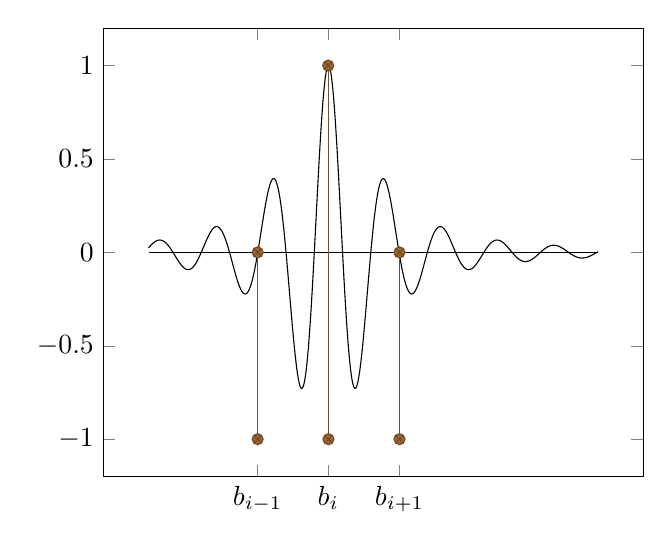
\begin{tikzpicture}
\begin{axis}[
	xticklabels = {$b_{i-1}$, $b_i$, $b_{i+1}$},
	xtick = {4.426, 5.995, 7.58},
	]
\addplot[
		domain = 2:12,
		]{0};
\addplot[
		domain = 2:12,
		samples = 1000,
		]{-sin(5*deg(x)-8.87)/((x-6)^2 + 1)};
\addplot+[
		ycomb,
		]coordinates{
		(4.426, 0) (5.995, 1) (7.58, 0)
		(4.426, -1) (6, -1) (7.58, -1)};
\end{axis}

\end{tikzpicture}
\end{center}

This is time consuming so the receiver instead constructs two Lagrange polynomials $Q$ and $E$, of degrees $n - 1 + e$ and $e$ respectively, such that 
$$\forall i\in[1..(n+2e)].(Q(i)\ =\ b_i E(i))$$
That is to say, E `blocks' the erroneous symbols by having roots at their values. If there are fewer than $e$ errors then $E$ may block some correct symbols but we still have many more than the $n+1$ values needed to define $P$. Now a system of linear equations can be formed to determine $Q$ and $E$ and work out the correct values of $P$.


\section{Signal \& Image Processing}

\subsection{Linear Algebra Foundation}

Scalar products:
\begin{align*}
	\mathcal{R}^n\ :&\ \vec{x}\cdot\vec{y}\ =\ \sum\limits_{i=1}^n x_iy_i \\
	\mathcal{C}^n\ :&\ \vec{x}\cdot\vec{Y}\ =\ \sum\limits_{i=1}^n x_i\bar{y_i}
\end{align*}

Normal length:
$$||\vec{x}||\ =\ \sqrt{\vec{x}\cdot\vec{x}}$$

\subsection{Basis Vectors}
A set of vectors ($b_1, b_2, ..., b_n$) form a basis for a space $X$ if they are linearly independent and any vector in $X$ can be written as $\sum\alpha_ib_i$. They are also considered orthonormal if the norm of all vectors with themselves is one and with all others is zero.

Now that for vector $x$ we have:
\begin{align*}
	b_ix\ &=\ b_i(\alpha_1 b_1 + \alpha_2b_2 + ... + \alpha_ib_i + ... + \alpha_nb_n ) \\
	&=\ \alpha_1 b_1b_i + \alpha_2b_2b_i + ... + \alpha_ib_ib_i + ... + \alpha_nb_nb_i \\
	&=\ \alpha_1*0 + \alpha_2*0 + ... + \alpha_i * 1 + ... + \alpha_n*0 \\
	&=\ \alpha_i \\
	x\ &=\ (b_1x)b_1 + (b_2x)b_2 + ... + (b_nx)b_n
\end{align*}

The most common basis vectors $e_x$ are equal to zero at positions that aren't equal to $x$ and one otherwise. There is also the complex basis $f$ where:
\begin{align*}
	f_1\ &=\ (w_n^0, w_n^1, w_n^2, ..., w_n^{n-1}) \\
	f_k\ &=\ (w_n^0, w_n^k, w_n^{2k}, ..., w_n^{k(n-1)})\\
	f_n\ &=\ (w_n^0, w_n^n, w_n^{2n}, ..., w_n^{n(n-1)})
\end{align*}

These vectors are orthonormal but not orthogonal. Thus any vector $\mathbf{c}$ can have its $\mathbf{\hat{c}} = (\langle \mathbf{c, \psi_m}\rangle)_m$ where $\mathbf{\hat{c}}_m$ is the DFT of $\mathbf{c}$ at $m$.


\subsection{Band-Limited Signals \texorpdfstring{$f(t)$}{f(t)} of finite energy}
From above, we have $\hat{f}(\omega) = 0$ if $|\omega|>B$ usually $B = \pi$. Now we can choose the time unit, $\tau$, so that that 20,000 hertz is that same as $\pi$ oscillation per $\tau$ seconds, or $\tau = \frac{1s * \pi}{20,000}$.

Band limited signals can be uniquely determined by a series of samples. Assume that $f(t)$ is a $\pi$-band limited signal of finite energy. Then 
$$f(t)\ =\ \sum\limits_{n=-\infty}^{\infty}f(n)\frac{sin(\pi*(t-n))}{\pi*(t-n)}$$
Since $\hat{f}(\omega)=0$ outside $(-\pi,\pi)$ we can extend it periodically and it can represented by its Fourier series:
$$\hat{f}(\omega)\ =\ \sum\limits_{k=-\infty}^{\infty}C_k*e^{i\omega k}$$

\subsubsection{Frequency Domain}
\subsubsection{Time Domain}

\subsection{Filters}
Now that we can represent band-limited as a Fourier transform we can process them. This may include boosting bass or removing 50kHz hum from power stations. In general a filter $L$ acts on a signal $f(t)$ and produces an output signal $L[f](t)$. A filter must be CLTI (continuous, linear, and time invariant).

\begin{align*}
	L[f(t)]\ &=\ L[\sum\limits_{m=-\infty}^{\infty}f(m)sinc(t-m)] \\
	&=\ L[\lim\limits_{n\to\infty}\sum\limits_{m=-n}^{n}f(m)sinc(t-m)] \\
	&=\ \lim\limits_{n\to\infty} L[\sum\limits_{m=-n}^{n}f(m)sinc(t-m)] \\
	&=\ \lim\limits_{n\to\infty}\sum\limits_{m=-n}^{n} f(m)L[sinc(t-m)] \\
	&=\ \lim\limits_{n\to\infty}\sum\limits_{m=-n}^{n} f(m)L[sinc](t-m) 
\end{align*}	

\section{MP3}


\section{Local Search}

Principles:
\begin{itemize}
	\item Define some neighbourhood relation between any two solutions based on the nature of the solution
	\item When checking solutions, only move from one solution to a ``neighbour'' of that solution
\end{itemize}

\subsection{The Metropolis Method}
Start from any solution $S_0$ then pick any state $\tilde{S}$ in its neighbourhood. Define $E(S)$ to be the cost of state $S$. For the second step $S_1$ towards our full solution we say

$$S_1 \gets \begin{cases} \tilde{S} & if E(S_0) > E(\tilde{S}) \\ \tilde{S} \textit{ with probability } e^{\frac{E(\tilde{S}) - E(S_1)}{kT}}&\textit{otherwise}\end{cases}$$

Where $k$ is some environmental constant and $T$ is some factor that corresponds to the likelihood of high cost solutions (corresponds to temperature in thermodynamics environments).

This situation allows us to make use of \textit{simulated annealing}, by starting with a very high $T$ then gradually decreasing. This method reduces the likelihood of getting stuck in local minima.

\subsection{Hopfield Neural Networks}
A Hopfield neural net is an attempt to explain human associative memory. Nodes are connected by edges with weights $w\in\mathbb{Z}$. The conditions are as follows:
\begin{itemize}
	\item Each node $u$ has a state $S_u$ that is either 0 or 1
	\item An edge $(u,v)$ is considered good if $w_{uv} * S_u * S_v < 0$
	\item A node will flip states if the sum of the weights of its good edges is less than the sum of the weights of its bad edges. I.e.
	$$\sum\limits_{(u,v) is good} w_{uv} < \sum\limits_{(u,v) is bad} w_{uv}$$
\end{itemize}
This will converge as when an unstable node flips, the sum of the good edges in the system increases. As the sum of the good edges cannot be larger than the sum of all the edges there is an upper limit and the system must converge before then.

\subsection{Maximum Cut}
Finding the min cut of a graph can be done in polynomial time, however finding the max cut is NP-hard. Our task is to assign each node into either set $A$ or set $B$ such that $\sum\limits{u\in A, v\in B} w_{uv}$ is maximised.

To start we define the trait $C_x$ such that:

$$C_x \gets \begin{cases}1 &\textit{if } x\in A \\ -1 &\textit{if } x\in B\end{cases}$$

And define any edge $(u, v)$ as good if $C_v*C_u < 0$. We also define a node as satisfied if the sum of all incoming `good' edges is greater than the sum of all income `bad' edges.

\subsubsection{Psuedo-Polynomial Time Algorithm}
Start with some random cut. One at a time move any unsatisfied nodes. This may disrupt the equilibrium of other nodes but as the only edges that are effected are the edges connected to the node we just moved, the total sum of the good weights has increased, while the total sum of bad weights has decreased.

Once this has converged we can say:
\begin{align*}
	\sum\limits_{u,v\in A} w_{uv} &\leq \sum\limits_{u,v \in A,B} w_{uv}\\
	\sum\limits_{u,v\in B} w_{uv} &\leq \sum\limits_{u,v \in A,B} w_{uv}\\
	\sum\limits_{u,v\in A} w_{uv} +  \sum\limits_{u,v\in B} w_{uv}&\leq 2\sum\limits_{u,v \in A,B} w_{uv} \\
	\sum\limits_{u,v\in A} w_{uv} +  \sum\limits_{u,v\in B} w_{uv}&\leq 2\sum\limits_{u,v \in A,B} w_{uv} \\
	\sum\limits_{(u,v)\in E} w_{uv} &\leq 2\sum\limits_{u,v \in A,B} w_{uv} 
\end{align*}

But the optimal solution is also less than  or equal to the total sum of all edges in the graph so we have
$$opt \leq 2\sum\limits_{u,v \in A,B} w_{uv}$$
Confirming that our solution is more than half of the optimal solution.

\subsubsection{Polynomial Time Algorithm}
By slightly lowering our lower bound from $\frac{opt}{2}$ to $\frac{opt}{2+\epsilon}$ we can create a polynomial time algorithm. Specifically we redefine a satisfied node to be on such that:

$$\sum\limits_{(u,v)\textit{ is bad}} < (1 + \frac{2\epsilon}{n})\sum\limits_{(u,v)\textit{ is good}} w_{uv}$$

After each swap the weight of all good edges is increased by $1+\frac{2\epsilon}{n}$, and after $\frac{n}{2\epsilon}$ swaps the weight of all good edges has increased by $(1 + \frac{2\epsilon}{n})^{\frac{n}{2\epsilon}}$. And because of math if $x > 1$ then $(x + \frac{1}{x})^x > 2$ and you can double at most $log(w)$ times where $w$ is the number of weights. Now we have that the algorithm is at most $O(\frac{2\epsilon}{n}log(w))$

\subsection{Nash Equilibria}
\begin{description}
	\item[Nash Equilibrium] no agent has an incentive to switch
	\item[Social Optimum] if total cost for all agents is as small as possible
\end{description}

A Nash equilibrium is not necessarily a social optimum. Say agents $A_1, ..., A_n$ need to go from a source to destinations $D_1, ..., D_n$. There is a direct path from the source to each $D_i$ with a cost of $\frac{1}{i}$ and also a path from the source to another node $N*$ with a cost of $1+\epsilon$ and paths from $N*$ to each destination with cost 0. The social optimum would be for all agents to split the cost of the path to node $N*$ and each pay $\frac{1+\epsilon}{n}$ for a total cost of $1+\epsilon$. However $A_n$ is now paying $\frac{\epsilon}{n}$ more than they need to otherwise so they would switch. All other agents are now paying $\frac{1+\epsilon}{n-1}$ so $A_{n-1}$ would now switch etc. The total cost is now $\sum\limits_{i=1}^{n}\frac{1}{i} \approx log(n)$

We can prove, however that a Nash equilibrium is not worse than $log(n)*opt$
	























































\end{document}
